\chapter{Arhitektura i dizajn sustava}
		
		Arhitektura se može podijeliti na dva podsustava:
	\begin{itemize}
		\item Mobilna aplikacija
		\item Baza podataka
	\end{itemize}
	
	\begin{figure}[h]
		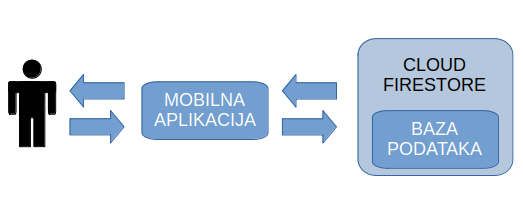
\includegraphics[scale=0.55]{slike/Arhitektura_sustava.PNG}
		\centering
		\caption{Arhitektura sustava}
		\label{fig:Arhitektura_sustava}
	\end{figure}
	
		\textit{\underbar{Mobilna aplikacija}} je program koji se izvodi na mobilnom uređaju. Mobilne aplikacije se uglavnom preuzimaju s distribucijskih platformi, nakon čega se provodi njihova instalacija. Korisnik koristi mobilnu aplikaciju za obrađivanje željenih zahtjeva, pri čemu aplikacija po potrebi pristupa bazi podataka.
		
		\textit{\underbar{Baza podatka}} je organizirani skup strukturiranih podataka. Za pohranu i pristup podacima koristi se računalni sustav.
		
		Za izradu naše mobilne aplikacije odabrali smo Flutter, softver za razvoj korisničkog sučelja otvorenog koda koji je stvorio Google. Razlog zbog kojeg smo odabrali Flutter je jednostavnost izrade aplikacija i mogućnost višeplatformskog razvoja korištenjem jednog koda. Još jedna velika prednost je to što se njime može realizirati i frontend i backend. Flutter koristi programski jezik Dart. Odabrano razvojno okruženje je Visual Studio Code.
		
		Baza podataka koju ćemo koristiti je Cloud Firestore. Cloud Firestore je NoSQL, dokumentno orijentirana baza podataka. Dokumenti su organizirani u kolekcije, a svaki dokument ima svoje ime (koje služi kao identifikator) i skup atributa kojima su pridružene vrijednosti. Glavne prednosti ovakve organizacije su efikasni upiti i velika brzina rada. Cloud Firestore omogućuje iOS, Android i web aplikacijama izravan pristup putem njihovih vlastitih programskih alata.
		
		Arhitektura sustava temeljiti će se na MVVM (Model-View-ViewModel) konceptu. Karakteristika MVVM koncepta je podjela na komponente, čiji nezavisni razvoj osigurava fleksibilnost, smanjuje međuovisnost, povećava ponovnu uporabivost i pojednostavljuje ispitivanje. \newline
		MVVM koncept se sastoji od:
	\begin{itemize}
		\item \textbf{\underline{Model}} - Pohranjuje podatke i informacije potrebne za rad aplikacije. Odvojen je od logičkog dijela koji određuje prikaz podataka i usluga koje njima manipuliraju.
		\item \textbf{\underline{View}} - Predstavlja sučelje koje korisnik vidi u interakciji s aplikacijom. Identificira i reagira na korisničke akcije.
		\item \textbf{\underline{ViewModel}} - Središnja komponenta sustava. Služi kao sučelje između Modela i Viewa. Šalje i prima podatke od Modela te osigurava podatke potrebne Viewu. Također promatra promjene koje se događaju u Viewu. Raspolaže metodama koje održavaju stanja Viewa i upravlja podacima u Modelu.
	\end{itemize}
		
	\eject

				
		\section{Baza podataka}
			
			\text Za potrebe našeg sustava koristit ćemo NoSQL bazu podataka orijentirana na dokumente, odnosno kolekcije dokumenata. Gradivna jedinka baze je dokument koji je definiran svojim imenom i skupom atributa. Zadaća baze podataka jest jednostavna i brza pohrana, izmjena i dohvat podataka za daljnju obranu. Baza podataka ove aplikacije sastoji se od dva entiteta, a to su:
			
			\begin{itemize}
				\item Korisnik
				\item Tečajevi
			\end{itemize}
		
			\subsection{Opis tablica}
			

				\textbf{Korisnik} \text    Ovaj entitet sadržava sve važne informacije o korisniku aplikacije. Sadrži atribute: about, cardExp, creditCard, firstName, iban, image, lastName, lecturer, mail, secCode, username. Za svakog novog registriranog korisnika kreira se dokument pod šifrom u bazi podataka.
				
				\begin{longtabu} to \textwidth {|X[6, l]|X[6, l]|X[20, l]|}
					
					\hline \multicolumn{3}{|c|}{\textbf{Korisnik}}	 \\[3pt] \hline
					\endfirsthead
					
					\hline \multicolumn{3}{|c|}{\textbf{Korisnik}}	 \\[3pt] \hline
					\endhead
					
					\hline 
					\endlastfoot
					
					Mail & string & mail korisnika \\ \hline
					Username & string & korisničko ime \\ \hline
					Lecturer & boolean & oznaka je li korisnik registriran kao predavač \\ \hline
					FirstName & string & ime korisnika \\ \hline
					LastName & string & prezime korisnika \\ \hline
					CardExp & string & datum isteka kartice za naplatu \\ \hline
					CreditCard & string & broj kartice za naplatu \\ \hline
					SecCode & string & kod za verifikaciju kartice \\ \hline
					iban & string & IBAN računa za isplatu honorara \\ \hline
					About & string & kratka biografija o korisniku ukoliko je predavač \\ \hline
					Image & & fotografija korisnika ukoliko je predavač \\ \hline
					
					
				\end{longtabu}
			
			\textbf{Tečajevi} \text    Ovaj entitet sadržava sve važne informacije o tečajevima koji su dostupni na aplikaciji. Sadrži atribut name te kolekciju za svaku razinu tečaja (beginner, intermediate, advanced) koja će sadržavati dodatne informacije o pojedinom tečaju. Za svaku kategoriju tečaja kreiran je dokument pod šifrom u bazi podataka, a za svaki tečaj kreira se dokument unutar kolekcije za odrabranu razinu i kategoriju tečaja. 
			
			\begin{longtabu} to \textwidth {|X[6, l]|X[6, l]|X[20, l]|}
				
				\hline \multicolumn{3}{|c|}{\textbf{Tečajevi}}	 \\[3pt] \hline
				\endfirsthead
				
				\hline \multicolumn{3}{|c|}{\textbf{Tečajevi}}	 \\[3pt] \hline
				\endhead
				
				\hline 
				\endlastfoot
				
				Name & string & naziv kategorije tečaja \\ \hline
				Razina tečaja & kolekcija & sadrži tri moguće razine tečajeva: početnička, srednja i napredna \\ \hline					
				
			\end{longtabu}
			
			
			\subsection{Dijagram baze podataka}
				
			
			\eject
			
			
		\section{Dijagram razreda}
		
			\textit{Potrebno je priložiti dijagram razreda s pripadajućim opisom. Zbog preglednosti je moguće dijagram razlomiti na više njih, ali moraju biti grupirani prema sličnim razinama apstrakcije i srodnim funkcionalnostima.}\\
			
			\textbf{\textit{dio 1. revizije}}\\
			
			\textit{Prilikom prve predaje projekta, potrebno je priložiti potpuno razrađen dijagram razreda vezan uz \textbf{generičku funkcionalnost} sustava. Ostale funkcionalnosti trebaju biti idejno razrađene u dijagramu sa sljedećim komponentama: nazivi razreda, nazivi metoda i vrste pristupa metodama (npr. javni, zaštićeni), nazivi atributa razreda, veze i odnosi između razreda.}\\
			
			\textbf{\textit{dio 2. revizije}}\\			
			
			\textit{Prilikom druge predaje projekta dijagram razreda i opisi moraju odgovarati stvarnom stanju implementacije}
			
			
			
			\eject
		
		\section{Dijagram stanja}
			
			
			\textbf{\textit{dio 2. revizije}}\\
			
			\textit{Potrebno je priložiti dijagram stanja i opisati ga. Dovoljan je jedan dijagram stanja koji prikazuje \textbf{značajan dio funkcionalnosti} sustava. Na primjer, stanja korisničkog sučelja i tijek korištenja neke ključne funkcionalnosti jesu značajan dio sustava, a registracija i prijava nisu. }
			
			
			\eject 
		
		\section{Dijagram aktivnosti}
			
			\textbf{\textit{dio 2. revizije}}\\
			
			 \textit{Potrebno je priložiti dijagram aktivnosti s pripadajućim opisom. Dijagram aktivnosti treba prikazivati značajan dio sustava.}
			
			\eject
		\section{Dijagram komponenti}
		
			\textbf{\textit{dio 2. revizije}}\\
		
			 \textit{Potrebno je priložiti dijagram komponenti s pripadajućim opisom. Dijagram komponenti treba prikazivati strukturu cijele aplikacije.}